% Copyright National ICT Australia 2005-2012
%	Author : Anthony Mak
%                Olivier Mehani
%		 William Uther
%
% This program can be redistributed and/or modified under the terms
% of the LaTeX Project Public License Distributed from CTAN
% archives in directory macros/latex/base/lppl.txt.

% If this template does not work, please check you have installed these.
% Required latex packages :-
%		Beamer class version 3.00 or higher
%		pgf version 0.63 or higher
%		xcolor version 2.00 or higher
%		(For details please read Beamer User Guide section 2.1 )
% Required NICTA Beamer Template files :-
%		(Make sure to include the following files in your TeX path)
%			beamerfontthemeNICTA.sty
%			beamercolorthemeNICTA.sty
%			beamercolorthemeNICTAsidebar.sty
%			beamerinnerthemeNICTA.sty
%			beamerouterthemeNICTA.sty
%			beamerthemeNICTA.sty

% /*** NO NEED TO MODIFY ***
\documentclass{beamer}
%\usetheme{NICTA}
%\usetheme[pagenum=false]{NICTA}
\usetheme[sidebar=false]{NICTA}

\usepackage[australian]{babel}
\graphicspath{{graphics/}}
% *** NO NEED TO MODIFY ***/
\usepackage[utf8]{inputenc}
\usepackage{times}
\usepackage{url}
\usepackage{latexsym}
\usepackage{graphicx}
\usepackage{color}
\usepackage{subfig}
%\usepackage{subcaption}
%\usepackage{pgfplotstable}
\usepackage{amssymb}
\usepackage{amsmath}
\usepackage[font={small}]{caption}



%%%%%%%%%%%%%%%%%%%%%%%%%%%%%%%%%
\newcommand{\RQ}[1][1]{\textbf{RQ#1}\xspace}

\newcommand{\figref}[2][]{Figure~\ref{#2}\xspace}
\newcommand{\tabref}[2][]{Table~\ref{#2}\xspace}

\newcommand{\lex}[1]{\textit{#1}\xspace}

\newcommand{\dataset}[1]{\texttt{#1}\xspace}
\newcommand{\EWT}{\dataset{EWT}}
\newcommand{\WSJ}{\dataset{WSJ}}
\newcommand{\Brown}{\dataset{Brown}}
\newcommand{\Reuters}{\dataset{Reuters}}
\newcommand{\MUC}{\dataset{MUC7}}

\newcommand{\method}[2][]{\ensuremath{\textsc{#2#1}}\xspace}
\newcommand{\unigram}[1][]{\method{Unigram}}
\newcommand{\brown}[1][]{\method[\ensuremath{_{#1}}]{Brown}}
\newcommand{\CW}[1][]{\method[#1]{CW}}
\newcommand{\CBOW}[1][]{\method[#1]{CBOW}}
\newcommand{\Skipgram}[1][]{\method[#1]{Skip-gram}}
\newcommand{\Glove}[1][]{\method[#1]{Glove}}
\newcommand{\withup}{\method{+UP}}

\newcommand{\task}[1]{\textsf{#1}\xspace}
\newcommand{\pos}{\task{POS tagging}}
\newcommand{\chunking}{\task{Chunking}}
\newcommand{\ner}{\task{NER}}
\newcommand{\mwe}{\task{MWE}}


\newcommand{\evmeasure}[1]{\textsc{#1}\xspace}
\newcommand{\accuracy}{\evmeasure{Acc}}
\newcommand{\fscore}{\evmeasure{F1}}
%%%%%%%%%%%%%%%%%%%%%%%%%%%%%%%%%%%

%%%%% TITLE SLIDE %%%%%

\title[Word Representations on Sequence Labelling Tasks] % (optional, use only with long paper titles)
{Big Data Small Data, In Domain Out-of Domain, Known Word Unknown
  Word: The Impact of Word Representations on Sequence Labelling Tasks}

\author[Lizhen Qu et al.]{\textbf{Lizhen Qu}, Gabriela Ferraro, Liyuan Zhou, Weiwei Hou, \\
Nathan Schneider \& Timothy Baldwin }


\begin{document}

{\setbeamertemplate{footline}{}
\begin{frame}
  \titlepage
\end{frame}
}





%%%%% FIRST SLIDE %%%%%
\section{Intro}
\label{sec:intro}



\begin{frame}
\frametitle{What we want to know about word embeddings}
  \framesubtitle{Research questions}

\begin{itemize}
\item[\bf RQ1:] Are word embeddings better than baseline approaches of one-hot unigram features and Brown clusters?
\item[\bf RQ2:] Do word embeddings require less training data than one-hot unigram features? If so, to what degree can word embeddings reduce the amount of labelled data?
\item[\bf RQ3:] What is the impact of updating word embeddings in sequence
  labelling tasks, both empirically over the target task and
  geometrically over the vectors?
\item[\bf RQ4:] What is the impact of these word embeddings (with and without
  updating) on both OOV items (relative to the training data) and
  out-of-domain data?
\item[\bf RQ5:] Are some word embeddings better than others in a sequence labelling context?
\end{itemize}
\end{frame}




\begin{frame}
\frametitle{Experiments Setup}
\framesubtitle{Fix the experiments conditions}
  
\begin{itemize}
\item[-] \textbf{Pre-trained word embeddings}
	\begin{itemize}			
		\item[-] Corpora 
			\begin{itemize}			
				\item[-] UMBC \cite{UMBC:2013}, 48.1GB 
				\item[-] One Billion \cite{OneBillion:2013}, 4.1GB 
				\item[-] English Wikipedia, 49.6GB 		
			\end{itemize}
		\item[-] Embedding dimensions: \ $d \in \{25, 50, 100, 200\}$
		\item[-] Context window size: $m \in \{1, 5, 10\}$	
	\end{itemize}
\item[-] \textbf{Selected Word Representations} 
	\begin{itemize}
		\item[-] Brown clustering \cite{Brown92class-basedn-gram}
		\item[-] CBOW ~\cite{Mikolov13},
		\item[-]	 Skipgram \cite{Mikolov13NIPS},
		\item[-]	 Global vectors \cite{pennington2014glove} 
	\end{itemize}  	
\item[-] \textbf{Four sequence labeling tasks}
	\begin{itemize}
		\item[-] POS-Tagging,
		\item[-] Chunking, 
		\item[-] NER, 
		\item[-]	 MWE (Multi-word Expressions identification)
	\end{itemize}  					
\end{itemize}      
\end{frame}





\begin{frame}
\frametitle{Training, development and test data} 

\begin{table}
\centering
\begin{tiny}
\begin{tabular}{@{}c@{~~}c@{~~}c@{~~}c@{~~}c@{~~}c@{}}
\hline
& \textbf{Training} & \textbf{Development} & \textbf{\textit{In-domain} Test} & \textbf{\textit{Out-of-domain} Test} \\ \hline
\textbf{\pos} & \WSJ Sec.\ 0-18  & \WSJ Sec.\ 19--21 & \WSJ Sec.\ 22--24 & \EWT  \\
\textbf{\chunking} & \WSJ & \WSJ (1K sentences) & \WSJ (CoNLL-00 test) & \Brown \\
\textbf{\ner} & \Reuters (CoNLL-03 train) & \Reuters (CoNLL-03 dev) & \Reuters (CoNLL-03 test) & \MUC  \\
\textbf{\mwe} & \EWT (500 docs) & \EWT (100 docs)  & \EWT (123 docs) & --- \\
\hline
\end{tabular}
\label{}
\end{tiny}
\end{table}
\end{frame}



%%%%%%%%%%%%%%%%%%%%%%%%%%%%
%%% HEATMAPS 
\begin{frame}[plain]

\frametitle{Results} 

\begin{enumerate}
\begin{small}
\item[\bf RQ1:] Word embeddings vs. one-hot unigram features vs. Brown clusters?
\item[\bf RQ2:] Do word embeddings require less training data than one-hot unigram features?
% If so, to what degree can word embeddings reduce the amount of labelled data?
\end{small}
\end{enumerate}

\vspace{-0.7cm}

\begin{columns}
  \column{.55\textwidth}
  \begin{figure}
    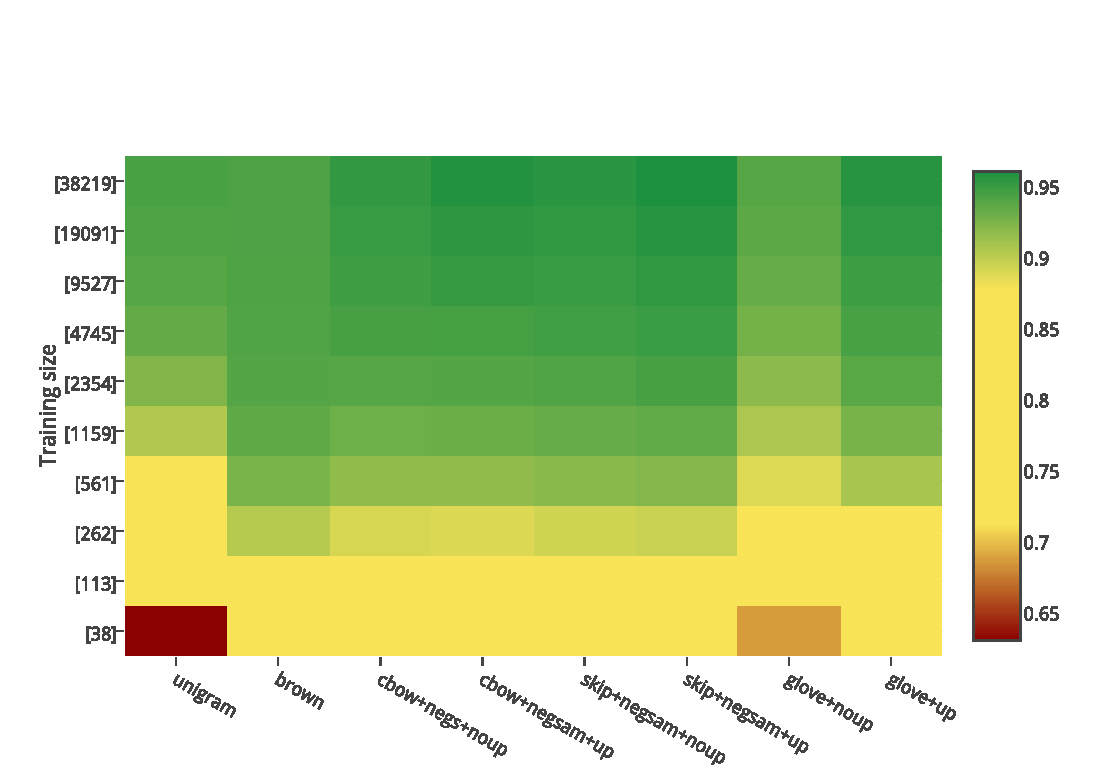
\includegraphics[scale=0.22]{../plots/map-pos-color-invert}    	   
    \caption{\pos (\accuracy)}	
	\vspace{-0.3cm}
    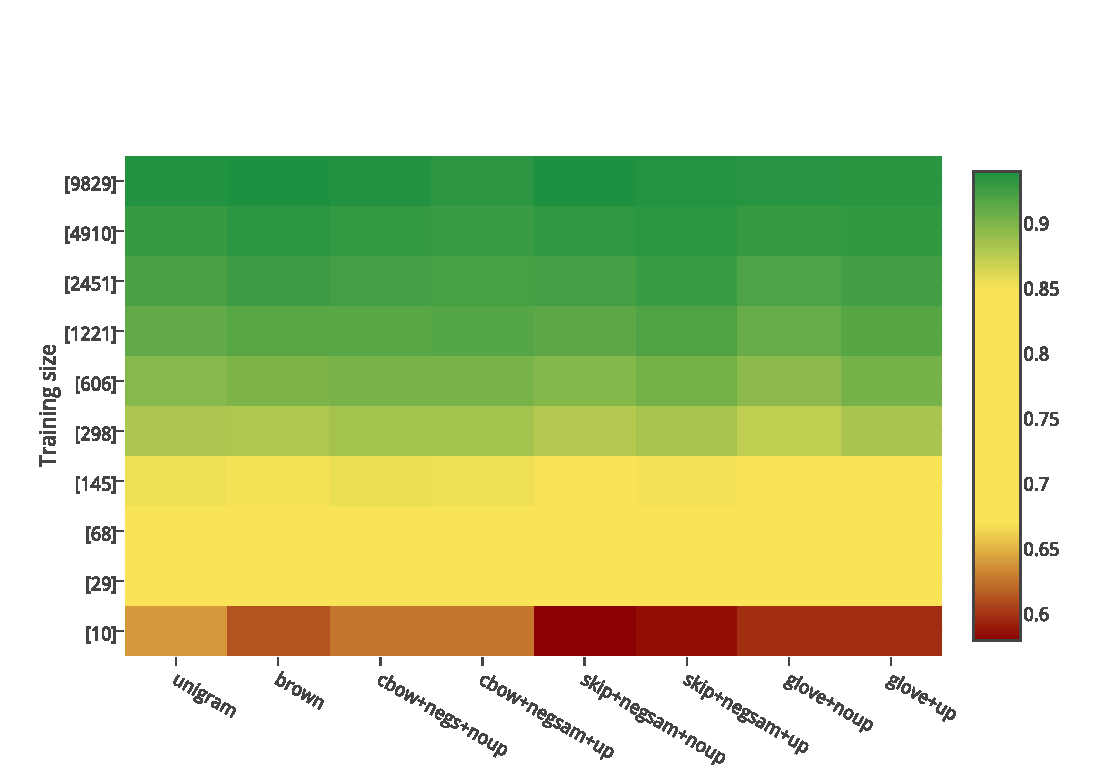
\includegraphics[scale=0.22]{../plots/map-chunk-color-invert}
   	\caption{\chunking (\fscore)}		
  \end{figure}  
  \column{.55\textwidth}
    \begin{figure}
    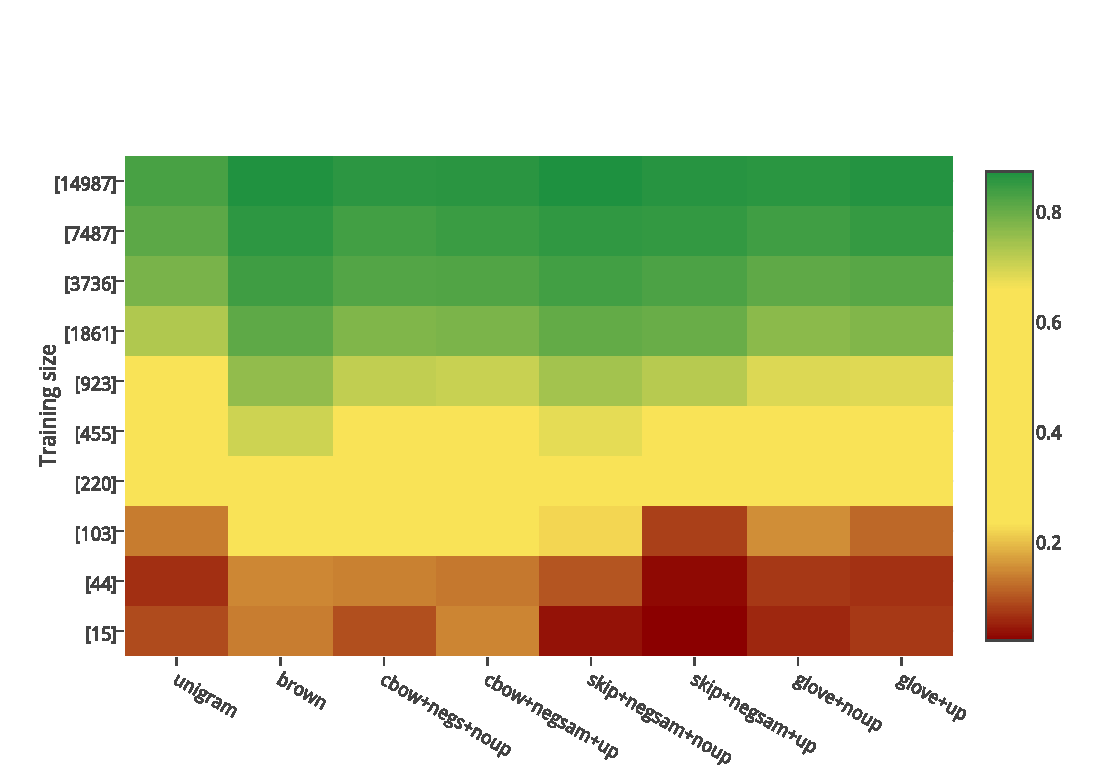
\includegraphics[scale=0.22]{../plots/map-ner-color-invert}    	
	\caption{\ner (\fscore)}	
	\vspace{-0.3cm}
    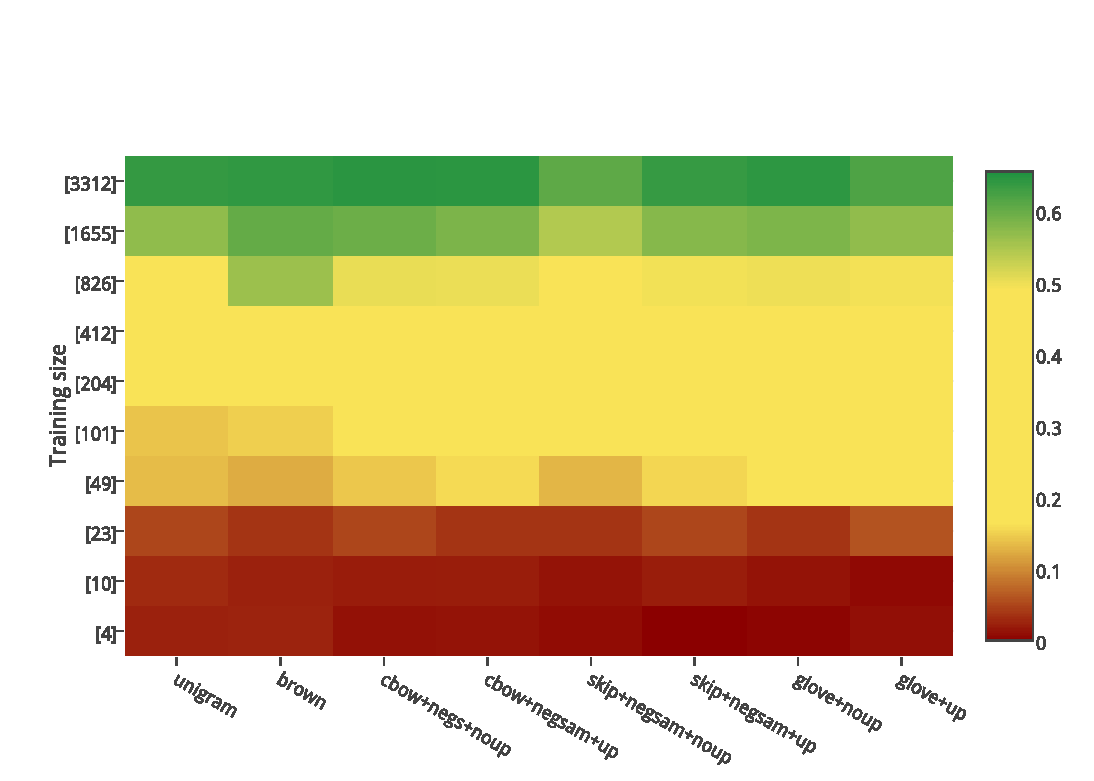
\includegraphics[scale=0.22]{../plots/map-mwe-color-invert}
	\caption{\mwe (\fscore)}	
     \end{figure}
\end{columns}
\end{frame}



%%%%%%%%%%%%%%%%%%%%%%%%%%%%
%%% Vector fields
\begin{frame}
\frametitle{}

\textbf{RQ3}: What is the impact of updating word embeddings geometrically over the vectors?

\begin{columns}	
	\column{.55\textwidth}
	  \begin{figure}
	   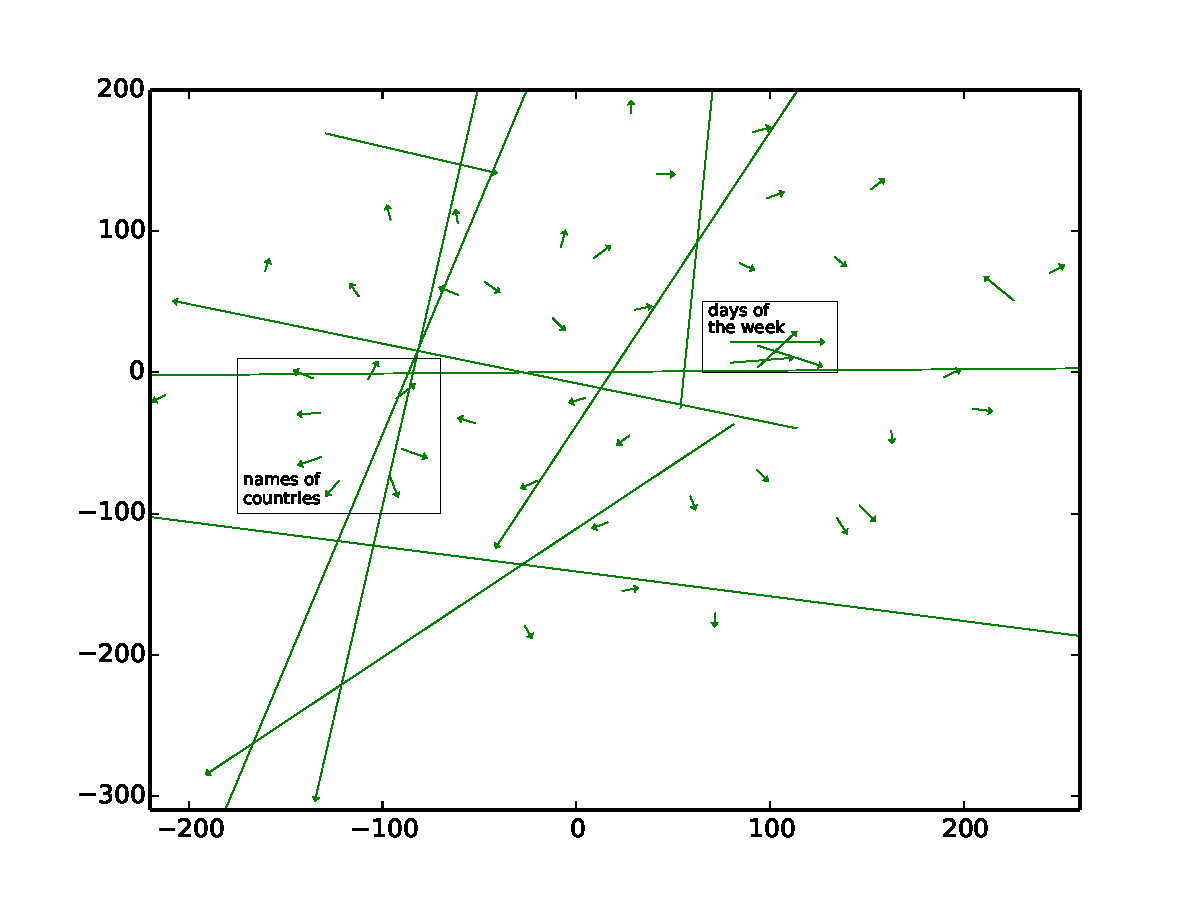
\includegraphics[width=\textwidth]{../plots/vectorField/Lizhen/scaled/Lizhen_skip_chunking}
	   \caption{\chunking with \Skipgram}
	   \end{figure}
  	\column{.55\textwidth}
	  \begin{figure}
	   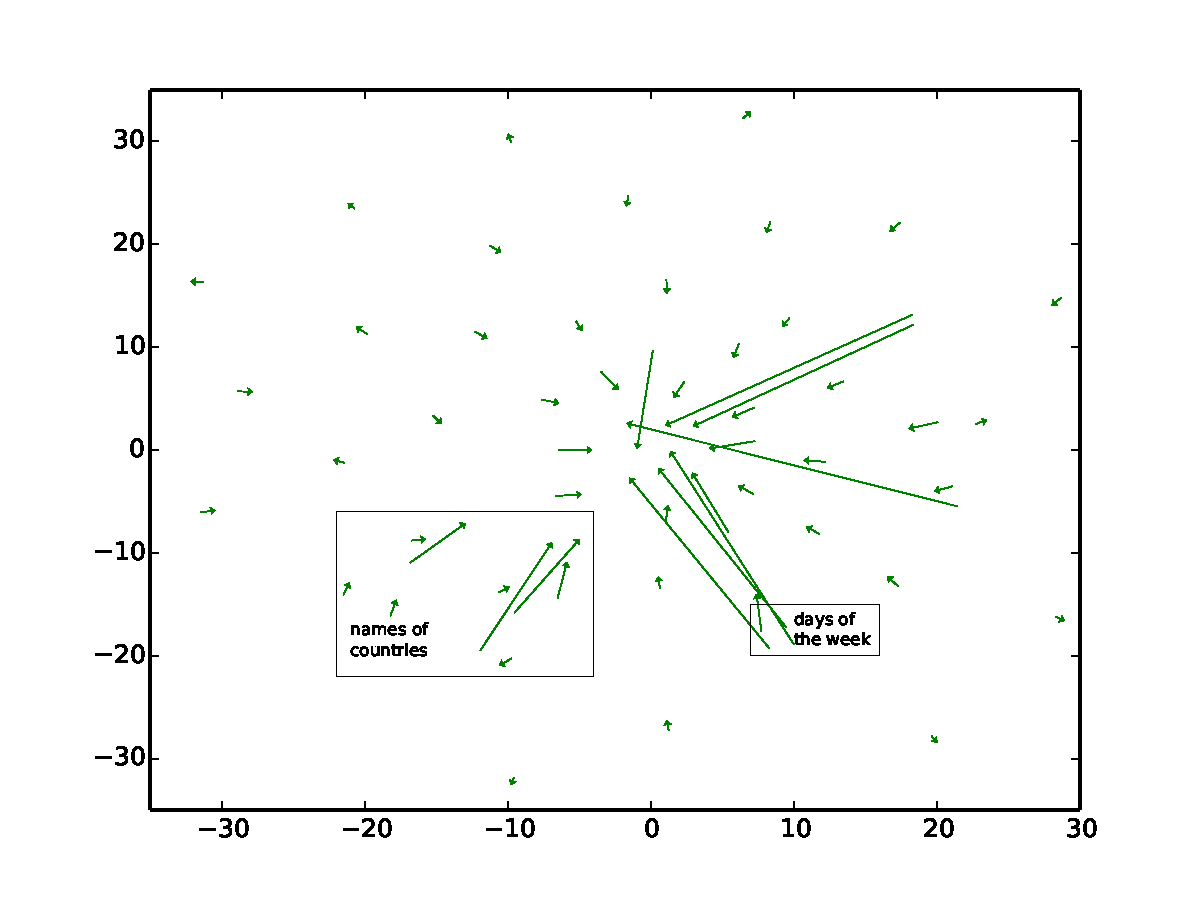
\includegraphics[width=\textwidth]{../plots/vectorField/Lizhen/Lizhen_skip_NER}    
   	    \caption{\ner with \Skipgram}
	   \end{figure}	    	
\end{columns}
\end{frame}



%%%%%%%%%%%%%%%%%%%%%%%%%%%%
%%% Plots
\begin{frame}
\frametitle{}

\begin{itemize}
\begin{small}
\item[\bf RQ4:] What is the impact of these word embeddings (with and without
  updating) on both OOV items (relative to the training data) and
  out-of-domain data?
\item[\bf RQ5:] Are some word embeddings better than others in a sequence labelling context?
\end{small}
\end{itemize}

\begin{figure}
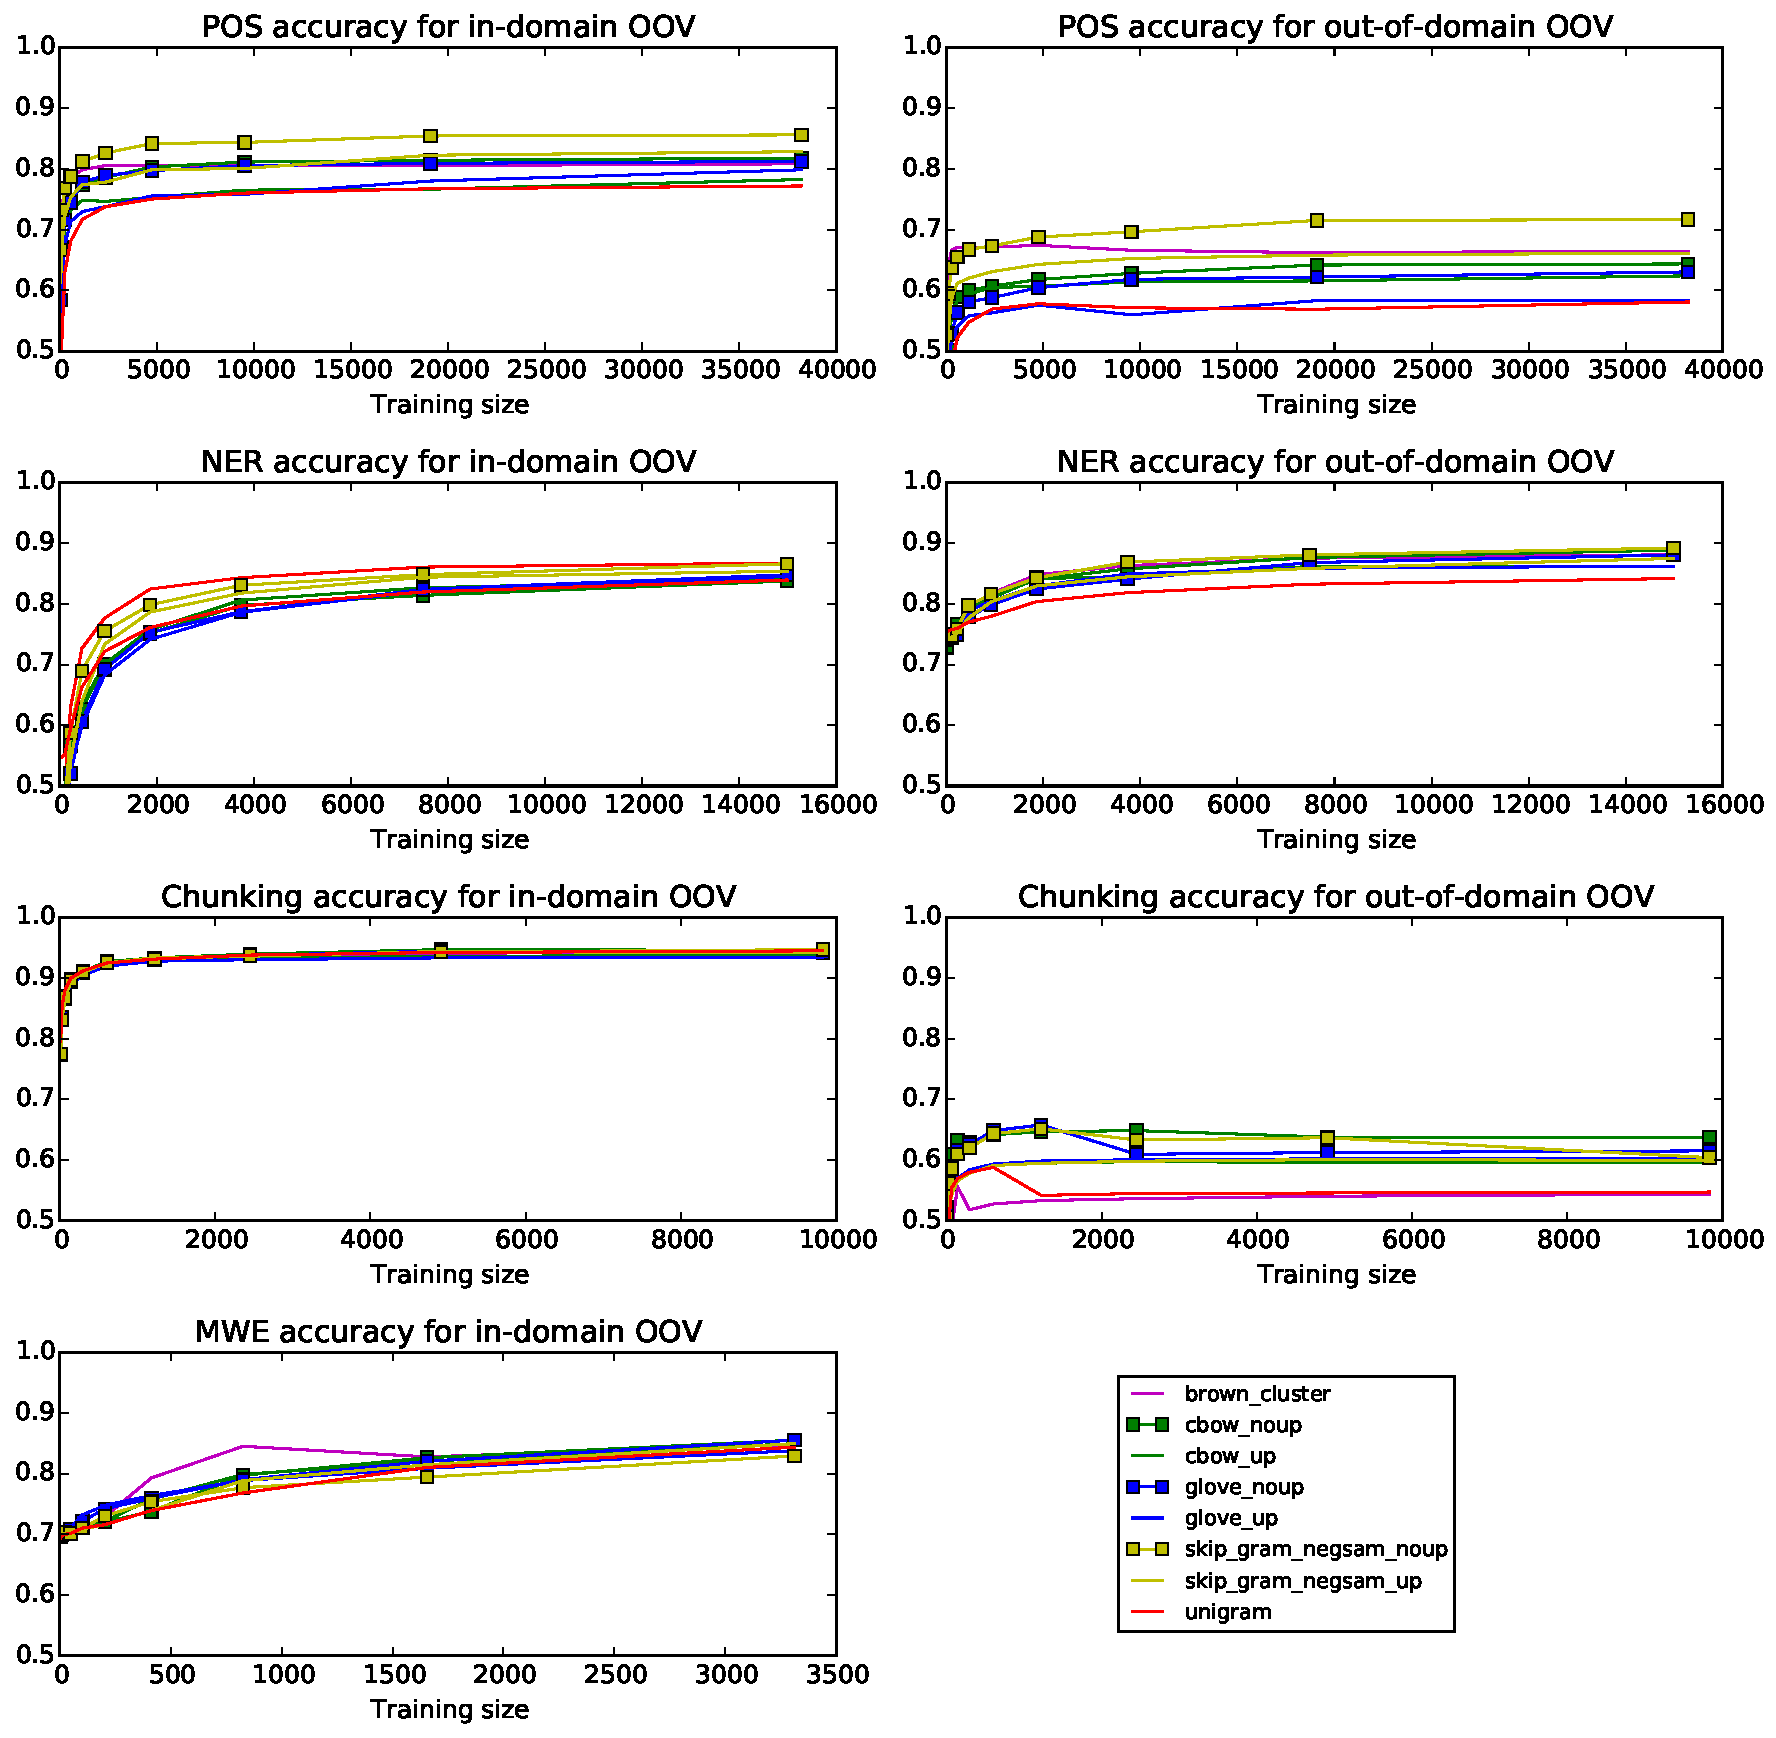
\includegraphics[scale=0.55]{../plots/OOV-plots}
\end{figure}	    	




\end{frame}


%%%%%%%%%%%%%%%%%%%%%%%
\bibliographystyle{acl2013}
\bibliography{../biblio}

\end{document}

